\documentclass[]{article}
\usepackage{lmodern}
\usepackage{amssymb,amsmath}
\usepackage{ifxetex,ifluatex}
\usepackage{fixltx2e} % provides \textsubscript
\ifnum 0\ifxetex 1\fi\ifluatex 1\fi=0 % if pdftex
  \usepackage[T1]{fontenc}
  \usepackage[utf8]{inputenc}
\else % if luatex or xelatex
  \ifxetex
    \usepackage{mathspec}
  \else
    \usepackage{fontspec}
  \fi
  \defaultfontfeatures{Ligatures=TeX,Scale=MatchLowercase}
\fi
% use upquote if available, for straight quotes in verbatim environments
\IfFileExists{upquote.sty}{\usepackage{upquote}}{}
% use microtype if available
\IfFileExists{microtype.sty}{%
\usepackage{microtype}
\UseMicrotypeSet[protrusion]{basicmath} % disable protrusion for tt fonts
}{}
\usepackage[margin=1in]{geometry}
\usepackage{hyperref}
\hypersetup{unicode=true,
            pdftitle={Figure Check},
            pdfauthor={J.P. Meagher},
            pdfborder={0 0 0},
            breaklinks=true}
\urlstyle{same}  % don't use monospace font for urls
\usepackage{graphicx,grffile}
\makeatletter
\def\maxwidth{\ifdim\Gin@nat@width>\linewidth\linewidth\else\Gin@nat@width\fi}
\def\maxheight{\ifdim\Gin@nat@height>\textheight\textheight\else\Gin@nat@height\fi}
\makeatother
% Scale images if necessary, so that they will not overflow the page
% margins by default, and it is still possible to overwrite the defaults
% using explicit options in \includegraphics[width, height, ...]{}
\setkeys{Gin}{width=\maxwidth,height=\maxheight,keepaspectratio}
\IfFileExists{parskip.sty}{%
\usepackage{parskip}
}{% else
\setlength{\parindent}{0pt}
\setlength{\parskip}{6pt plus 2pt minus 1pt}
}
\setlength{\emergencystretch}{3em}  % prevent overfull lines
\providecommand{\tightlist}{%
  \setlength{\itemsep}{0pt}\setlength{\parskip}{0pt}}
\setcounter{secnumdepth}{0}
% Redefines (sub)paragraphs to behave more like sections
\ifx\paragraph\undefined\else
\let\oldparagraph\paragraph
\renewcommand{\paragraph}[1]{\oldparagraph{#1}\mbox{}}
\fi
\ifx\subparagraph\undefined\else
\let\oldsubparagraph\subparagraph
\renewcommand{\subparagraph}[1]{\oldsubparagraph{#1}\mbox{}}
\fi

%%% Use protect on footnotes to avoid problems with footnotes in titles
\let\rmarkdownfootnote\footnote%
\def\footnote{\protect\rmarkdownfootnote}

%%% Change title format to be more compact
\usepackage{titling}

% Create subtitle command for use in maketitle
\newcommand{\subtitle}[1]{
  \posttitle{
    \begin{center}\large#1\end{center}
    }
}

\setlength{\droptitle}{-2em}
  \title{Figure Check}
  \pretitle{\vspace{\droptitle}\centering\huge}
  \posttitle{\par}
  \author{J.P. Meagher}
  \preauthor{\centering\large\emph}
  \postauthor{\par}
  \predate{\centering\large\emph}
  \postdate{\par}
  \date{9 January 2018}

\usepackage{tikz}
\usepackage{pgfplots}
\usepackage{float}

\begin{document}
\maketitle

\section{Introduction}\label{introduction}

We are given a dataset of \(N\) bat echolocation call recordings denoted
\(\{y_n\}_{n = 1}^N\). This recording is then processed to produce a set
of smooth surfaces over a regular grid denoted
\(\{\tilde{S}_n\}_{n=1}^{N}\). This surface is produced by smoothing the
call spectrogram and mapping it to a regular grid over relevant
frequencies and an absolute time scale.

\begin{figure}
\centering
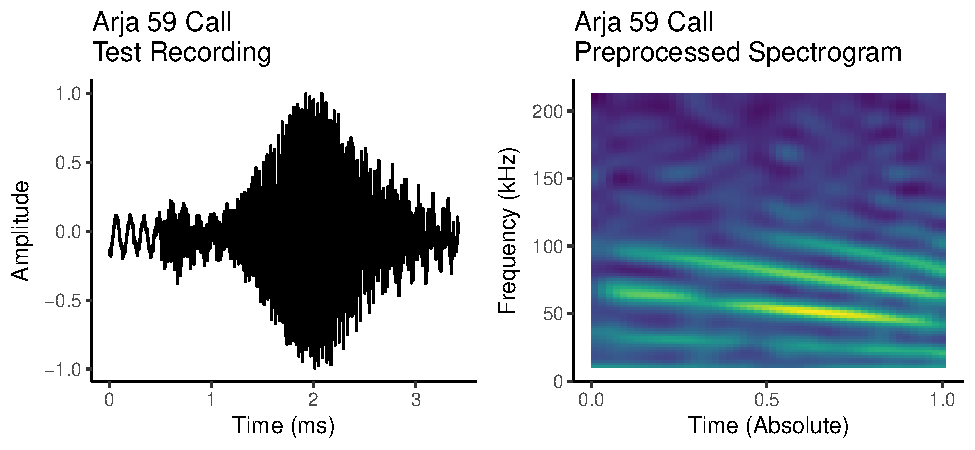
\includegraphics{figure_test_files/figure-latex/recording figure-1.pdf}
\caption{A randomly selected bat call from the species Arja alongside
it's corresponding smoothed surface representation.}
\end{figure}

Along with this dataset we are given a phylogeny defining the
evolutionary relationships between the species of bat.

\begin{figure}
\centering
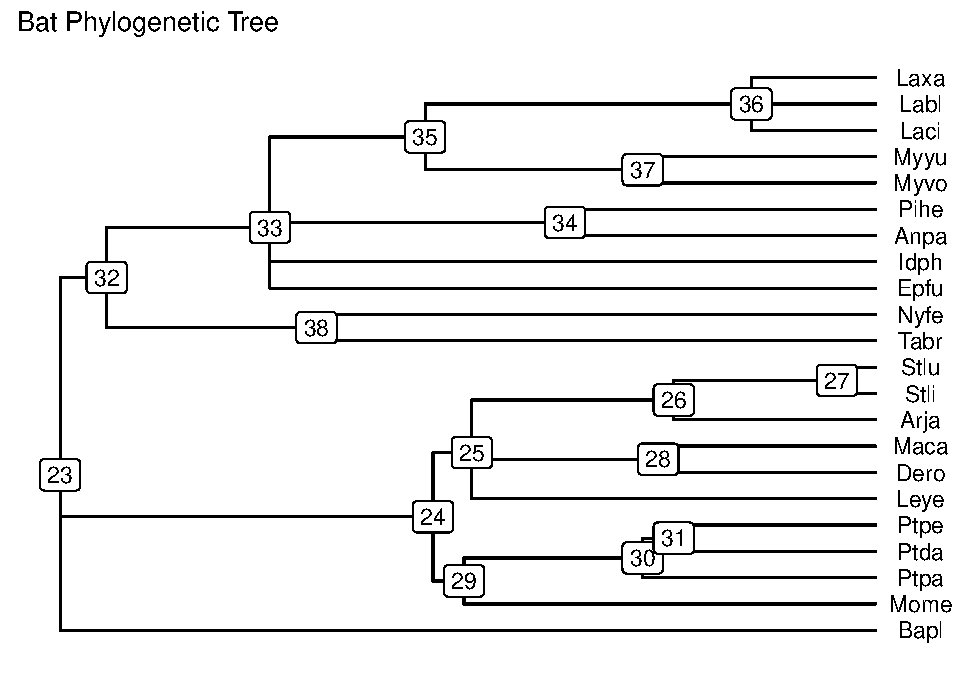
\includegraphics{figure_test_files/figure-latex/phylogeny figure-1.pdf}
\caption{Tree of assumed evolutionary relationships between Bat Species}
\end{figure}

Thus, for the dataset of Mexican Bat echolocation calls and the given
Phylogeny, Ancestral Reconstruction has been performed.

\section{The Current Model}\label{the-current-model}

\begin{figure}[htbp]
\centering
\begin{tikzpicture}[node distance = 2cm]

  \tikzstyle{rv} = [circle, draw]
    \tikzstyle{plate} = [node distance = 1.25cm]
    
    \node[rv, fill = gray!50, label = above left:$y_n$] (y) {};
    \node[rv, fill = gray!50, label = above left:$S_n$, right of = y] (S) {}
    edge[->] (y);
    
    \node[plate, above right of = S] (ntop) {};
    \node[plate, below left of = y, label = 5:$N$, ] (nbot) {};
    \draw[rounded corners] (ntop) rectangle (nbot) ;
    
    \node[rv, right of=S, label = above right:$\mathbf{w}$] (w) {}
    edge[->] (S);
    \node[above of = w, label = above right:$\Theta$] (theta) {\textbullet}
    edge [->] (w);
    \node[right of = w, label = above right:$\mathcal{P}$] (P) {\textbullet}
    edge [->] (w);
    \node[below of = w, label = above right:$\Phi$] (phi) {\textbullet}
    edge [->] (S);
    
    \node[plate, above right of = theta] (qtop) {};
    \node[plate, below left of = phi, label = 5:$Q$, ] (qbot) {};
    \draw[rounded corners] (qtop) rectangle (qbot);
    
    \node[rv, below of=S, label = below left:$\hat{S}$] (hatS) {}
    edge[<-] (w)
    edge[<-] (phi);
    \node[rv, below of=y, label = below left:$\hat{y}$] (haty) {}
    edge[<-] (hatS);
\end{tikzpicture}
\caption{A Graphical model detailing the structure of the model for evolution used to produce reconstructions of ancestral bat echolocation calls.}
\end{figure}


\end{document}
